\documentclass[11pt]{beamer}
\usetheme{PaloAlto}

\usepackage[utf8]{inputenc}
\usepackage[T1]{fontenc}
\usepackage{amsmath}
\usepackage{amsfonts}
\usepackage{amssymb}
\usepackage{forest}
\usepackage{url}

\setbeamercolor{logo}{bg=white}

\author{Christoph Teichmann \and Antoine Venant}
\title{Markov Chain Monte Carlo Methods}

\subtitle{}

\logo{
\includegraphics[height=0.65cm]{SaarLogo}}

\institute{}

\date{}

\subject{}

\setbeamercovered{invisible}

\setbeamertemplate{navigation symbols}{}

\begin{document}
	\centering
	
	\AtBeginSection[]{
		\begin{frame}
			\vfill
			\centering
			\begin{beamercolorbox}[sep=8pt,center,shadow=true,rounded=true]{title}
				\usebeamerfont{title}\insertsection\par%
			\end{beamercolorbox}
			\vfill
		\end{frame}
	}
	
	\begin{frame}
		\maketitle
	\end{frame}
	
	\section{Goals}
	
	\begin{frame}{Teaching Goals}
		\begin{itemize}
			\item Problem of Bayesian Inference
			\item Markov Chain Monte Carlo
			\item Metropolis-Hasting Technique
			\item Gibbs Technique
		\end{itemize}
	\end{frame}
	
	\section{Motivation}
	
	\begin{frame}{Our Model From Last Session}
		We were discussing how to learn a language model:
		
		\vspace{10pt} \begin{itemize}
			\item Bigram model for text
			\item Probabilities are hidden variables
			\item Dirichlet Prior for probabilities
		\end{itemize}
		
		\vspace{10pt} Can we improve this model?
	\end{frame}
		
	\begin{frame}{Hidden States}
		\centering
		Assume the words are generated from hidden states
		
		\vspace{10pt}
		\begin{itemize}
			\item $h \in H$ hidden tags
			\item $w \in L$ words
			\item $P_w$ distribution over words give hidden tags (one per tag)
			\item $P_h$ distribution over hidden tags given previous tag (one per tag) and initial tag
			\item $P_w$ and $P_h$ have Dirichlet Prior
		\end{itemize}
		
		$$P(w_1,w_2,\dots) = P(P_h)P(P_w) P_h(h_0) \prod_{i \in 1,\dots} P(w_i|h_i)P_h(h_i|h_{i-1})$$
	\end{frame}
	
	\begin{frame}{Make This Concrete}
		
		\begin{itemize}
			\item<1-> $L = \{\mbox{Mary, sees, something, ., John}\}$
			\item<1-> $H = \{1,2\}$
			\item<1-> how many probability distributions/densities are we thinking about?
			\item<2-> we need $2$ word given state, $2$ state given state, $1$ initial state + priors for each $\rightarrow$ $10$
			\item<2-> $\alpha$ for all parameters is $0.5$ except:
			\item<2-> $\alpha_{Mary}^1 = 1$, $\alpha_{sees}^2 = 1$ (symmetry breaking)
		\end{itemize}
		
		
		\vspace{10pt}Reminder: Dirichlet = $P(P_x) = \frac{\prod_{o \in O} P_x(o)^\alpha_o}{B(\boldsymbol{\alpha})}$
	\end{frame}
	
	
	\begin{frame}{Reasoning Based on the Model}
		Assume corpus: $C =$ ``Mary sees something''
		
		\vspace{10pt}\begin{itemize}
			\item What is posterior probability $P(P_{h}^{exam} | C)$, with:
				\begin{itemize}
					\item $P_{h}^{exam}(1|1) = 0.1$
					\item $P_{h}^{exam}(2|1) = 0.9$
					\item $P_{h}^{exam}(1|2) = 0.6$
					\item $P_{h}^{exam}(2|1) = 0.4$
					\item $P_{h}^{exam}(1|s) = 0.8$
					\item $P_{h}^{exam}(2|s) = 0.2$
				\end{itemize}
			\item What is $P(h_2 = 2)$?
			\item What is \dots
		\end{itemize}
	\end{frame}
	
	\begin{frame}{We Can Use Knowledge of Dirichlet}
		Easy if we know the tags, e.g.:
		
		\vspace{10pt} ``Mary:1 sees:2 something:1''
		
		\begin{align*}
			P(P_{h}^{exam}|T,C) & = & \frac{\prod_{i \in \{1,2\}} P_{h}^{exam}(i|1)^{\alpha_{i}^1}}{B(\boldsymbol{\alpha^1})} \\
			& & \times \frac{\prod_{i \in \{1,2\}} P_{h}^{exam}(i|2)^{\alpha_{i}^2}}{B(\boldsymbol{\alpha^2})} \\
			& & \times \frac{\prod_{i \in \{1,2\}} P_{h}^{exam}(i|s)^{\alpha_{i}^s}}{B(\boldsymbol{\alpha^s})}
		\end{align*}
		
		\vspace{10pt}
		Where $\alpha_{1}^s = 1.5$, $\alpha_{2}^1 = 1.5$, $\alpha_{1}^2 = 1.5$ and other $\alpha$s for hidden tags are still $0.5$
	\end{frame}
	
	\begin{frame}{But We do not Know the Hidden Tags}
		
		\begin{align*}
			P(P_{h}^{exam}|C) & = & \sum_{T} P(P_{h}^{exam}|T,C) P(T|C) \\
			& = & \sum_{T} P(P_{h}^{exam}|T,C) \frac{P(C|T)P(T)}{P(C)}
		\end{align*}
	\end{frame}
	
	
	\begin{frame}{Typical Problems in Bayesian Learning / Inference }
		$$P(P_{h}^{exam}|C) = \overbrace{\sum_{T}}^{\substack{\mbox{annoying} \\ \mbox{sum}}} P(P_{h}^{exam}|T,C) \frac{P(C|T)P(T)}{\overbrace{P(C)}^{\substack{\mbox{normalization factor} \\ \mbox{(secretly annoying sum)}}}}$$
		
		\vspace{10pt} We need a generic fix for this problem!
	\end{frame}
	
	\begin{frame}{Use Representatives}
		When you want to know what people think, you do not ask everyone, you ask a few representatives.\\[10pt]
		When you have an annoying some over $T$ you do not consider every possible asignment of tags, you only consider a few representative ones.
	\end{frame}
	
	\begin{frame}{What Does it Mean to be Representative}
		Let us make our problem more general:
		
		\begin{align*}
			P(P_{h}^{exam}|C) & = & \sum_{T} P(P_{h}^{exam}|T,C) \frac{P(C|T)P(T)}{P(C)} \\
			& & \overbrace{\sum_{V}}^{\substack{\mbox{sum over}\\\mbox{variable}}} \overbrace{f(V)}^{\substack{\mbox{function} \\ \mbox{of variable}}} \overbrace{P(V)}^{\substack{\mbox{probability} \\ \mbox{of variable}}}
		\end{align*}
		
		\vspace{10pt} Expected value problem -- Many problems in Bayesian Learning/Inference can be formulated as expected value problems
	\end{frame}
	
	
	\begin{frame}{The Law of Large Numbers}
		The law of large numbers can be formulated as follows:
		
		\begin{itemize}
			\item Produce sequence $V_1,V_2,\dots$
			\item $P(V_i = v)$ given by $P(V)$ from our expected value
			\item Then $\lim_{n \rightarrow \infty} \sum_{n} \frac{1}{n} f(v_i) = \sum_{V} f(V) P(V)$
		\end{itemize}
	\end{frame}
	
	\begin{frame}{What Does it Mean to be Representative?}
		We will try to generate a sequence as if each $v_i$ was drawn from $P(V)$
		
		\vspace{10pt} But how do we do this?
	\end{frame}
	
	\begin{frame}{For Simple Cases}
		For simple distributions (categorial) solutions exist based on pseudo-random number generators.
		
		\vspace{10pt} But we have a hard case here!
	\end{frame}
	
	\section{Markov Chains}
	
	\begin{frame}{Markov Chain Trick}
		\begin{itemize}
			\item  Produce a Markov Chain (later)
			\item  Produce sequence $V_1,V_2,\dots$ from Markov Chain
			\item Ensure certain conditions
			\item Then $\lim_{n \rightarrow \infty} \sum_{n} \frac{1}{n} f(v_i) = \sum_{V} f(V) P(V)$
		\end{itemize}
	\end{frame}
	
	\begin{frame}{What is a Markov Chain}
		\begin{itemize}
			\item Set of states $V$ -- will be variables of interest, can be infinite (but we assume discrete)
			\item Initial Probability $S(V_0)$
			\item Transition Probability $T(V_i|v_{i-1})$
		\end{itemize}
	\end{frame}
	
	\begin{frame}{Example}
		How to create $v_1,v_2,\dots$ from this:
		
		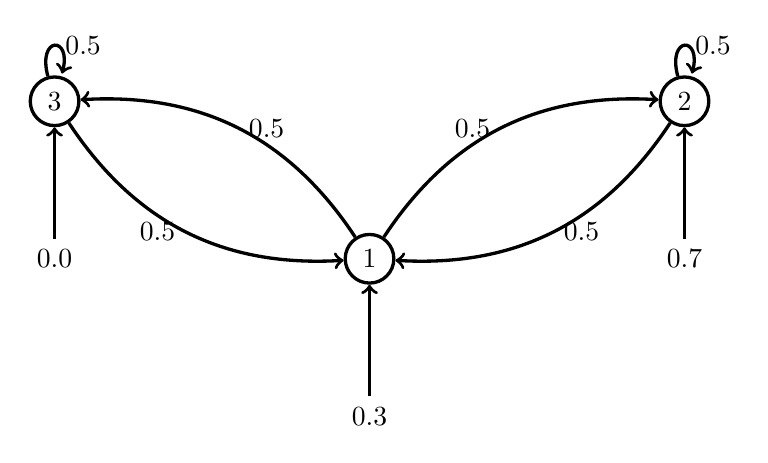
\begin{tikzpicture}[very thick]
			\node[draw,circle] (1) at (0,0) {1};
			\node[draw,circle] (2) at (4,2) {2};
			\node[draw,circle] (3) at (-4,2) {3};
			
			\node (11) at (0,-2) {0.3};
			\node (22) at (4,0) {0.7};
			\node (33) at (-4,0) {0.0};
			
			\path[draw,->] (11) edge (1);
			\path[draw,->] (22) edge (2);
			\path[draw,->] (33) edge (3);
			
			\path[draw,->] (1) edge[bend left] node[left] {0.5} (2) edge[bend right] node[right] {0.5} (3);
			
			\path[draw,->] (2) edge[bend left] node[right] {0.5} (1) edge[loop above] node[right] {0.5} (2);
			
			\path[draw,->] (3) edge[bend right] node[left] {0.5} (1) edge[loop above] node[right] {0.5} (3);
		\end{tikzpicture}
	\end{frame}
	
	\begin{frame}{What are the Magic Requirements?}
		What do we need so: $\lim_{n \rightarrow \infty} \sum_{n} \frac{1}{n} f(v_i) = \sum_{V} f(V) P(V)$?
	\end{frame}
	
	\begin{frame}{Magic Requirement 1: Invariant Distribution}
		Invariant distribution $I(V)$ of chain $= P(V)$
		
		\vspace{10pt} What is invariant distribution?
	\end{frame}
	
	\begin{frame}{Magic Requirement 1: Invariant Distribution}
		Invariant distribution $I(V)$ of chain $=P(V)$
		
		\vspace{10pt} $I(V)$ s.t. for all $v$: $I(v) = \sum_{v' \in V} T(v|v')I(v')$
		
		\vspace{10pt} Initial probability does not matter
	\end{frame}
	
	\begin{frame}{Example}
		$I(1) = I(2) = I(3) = \frac{1}{3} $ -- Show!
		
		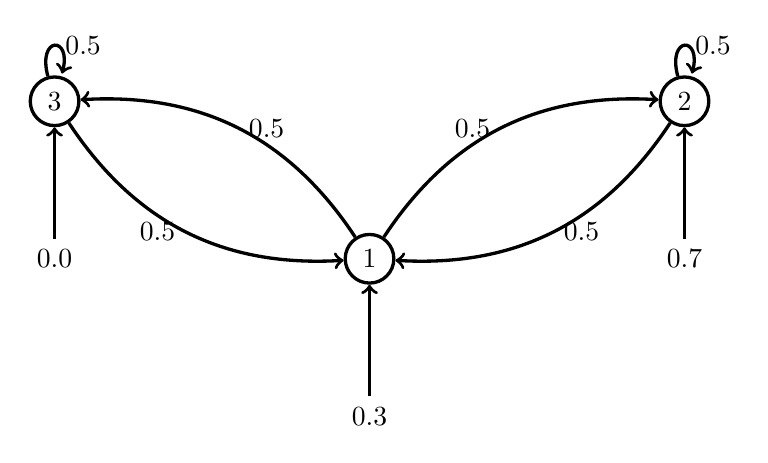
\begin{tikzpicture}[very thick]
		\node[draw,circle] (1) at (0,0) {1};
		\node[draw,circle] (2) at (4,2) {2};
		\node[draw,circle] (3) at (-4,2) {3};
		
		\node (11) at (0,-2) {0.3};
		\node (22) at (4,0) {0.7};
		\node (33) at (-4,0) {0.0};
		
		\path[draw,->] (11) edge (1);
		\path[draw,->] (22) edge (2);
		\path[draw,->] (33) edge (3);
		
		\path[draw,->] (1) edge[bend left] node[left] {0.5} (2) edge[bend right] node[right] {0.5} (3);
		
		\path[draw,->] (2) edge[bend left] node[right] {0.5} (1) edge[loop above] node[right] {0.5} (2);
		
		\path[draw,->] (3) edge[bend right] node[left] {0.5} (1) edge[loop above] node[right] {0.5} (3);
		\end{tikzpicture}
	\end{frame}
	
	\begin{frame}{Magic Requirement 2: Irreducibility}
		Irreducible: Same $I(v)$, no magic!
		
		\begin{tikzpicture}[very thick]
			\node[draw,circle] (1) at (0,0) {1};
			\node[draw,circle] (2) at (4,2) {2};
			\node[draw,circle] (3) at (-4,2) {3};
		
			\node (11) at (0,-2) {0.0};
			\node (22) at (4,0) {0.0};
			\node (33) at (-4,0) {1.0};
		
			\path[draw,->] (11) edge (1);
			\path[draw,->] (22) edge (2);
			\path[draw,->] (33) edge (3);
		
			\path[draw,->] (1) edge[loop above] node[right] {1.0} (1);
			
			\path[draw,->] (2) edge[loop above] node[right] {1.0} (2);
			
			\path[draw,->] (3) edge[loop above] node[right] {1.0} (3);
		\end{tikzpicture}
	\end{frame}
	
	\begin{frame}{Magic Requirement 3: Recurrence}
		Probability of returning is 1 -- always true for finite.
		
		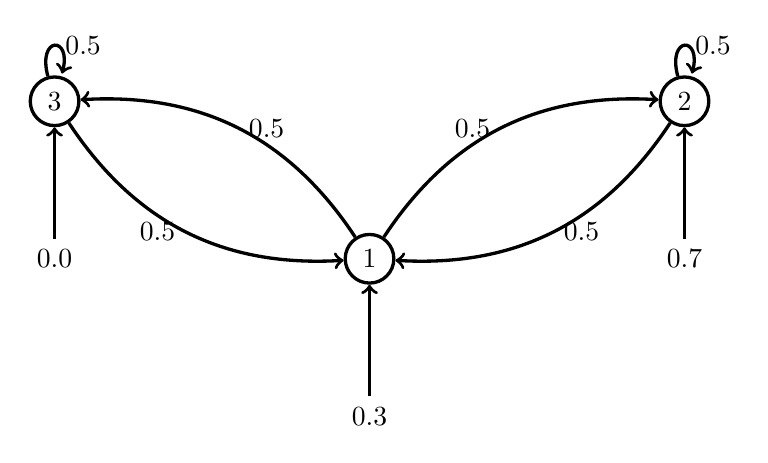
\begin{tikzpicture}[very thick]
		\node[draw,circle] (1) at (0,0) {1};
		\node[draw,circle] (2) at (4,2) {2};
		\node[draw,circle] (3) at (-4,2) {3};
		
		\node (11) at (0,-2) {0.3};
		\node (22) at (4,0) {0.7};
		\node (33) at (-4,0) {0.0};
		
		\path[draw,->] (11) edge (1);
		\path[draw,->] (22) edge (2);
		\path[draw,->] (33) edge (3);
		
		\path[draw,->] (1) edge[bend left] node[left] {0.5} (2) edge[bend right] node[right] {0.5} (3);
		
		\path[draw,->] (2) edge[bend left] node[right] {0.5} (1) edge[loop above] node[right] {0.5} (2);
		
		\path[draw,->] (3) edge[bend right] node[left] {0.5} (1) edge[loop above] node[right] {0.5} (3);
		\end{tikzpicture}
	\end{frame}
	
	\begin{frame}{Markov Chain Trick}
		\begin{itemize}
			\item  Produce a Markov Chain
			\item  Produce sequence $V_1,V_2,\dots$ from Markov Chain
			\item If Markove Chain Recurrent, Irreducible, and has Invariant Distribution $I(V) = P(V)$
			\item Then $\lim_{n \rightarrow \infty} \sum_{n} \frac{1}{n} f(v_i) = \sum_{V} f(V) P(V)$ 
			\item[] See "Markov Chains" by James Norris
			\item[] relevant chapters available online \url{http://www.statslab.cam.ac.uk/~james/Markov/})
		\end{itemize}
	\end{frame}
	
	\section{Invariant Tricks}
	
	\begin{frame}{How the Magic Happens}
		\begin{itemize}
			\item Irreducibility and Recurrence -- no general trick -- often easy
			\item Correct Invariant Distribution -- super hard?
		\end{itemize}
	\end{frame}
	
	\begin{frame}{Invariant Distribution Trick 1: Metropolis-Hastings}
		\begin{itemize}
			\item Proposal Distribution -- $p(V|v_i)$
			\item Must be easy to draw from!
			\item e.g. for example: flip one tag at random (table)
			\item Then accept with probability:
				$$T(v_i|v_{i-1}) = \min\left(1,\frac{P(v_i)p(v_{i-1}|v_i)}{P(v_{i-1})p(v_i|v_{i-1})}\right)$$
			\item Otherwise $v_i = v_{i-1}$
		\end{itemize}
	\end{frame}
	
	\begin{frame}{Invariant Distribution Trick 1: Metropolis-Hastings}
		\begin{itemize}
			\item Proposal Distribution -- $p(V|v_i)$
			\item Must be easy to draw from!
			\item e.g. for example: flip one tag at random (table)
			\item Then accept with probability:
				$$T(v_i|v_{i-1}) = \min\left(1,\frac{P(v_i)p(v_{i-1}|v_i)}{P(v_{i-1})p(v_i|v_{i-1})}\right)$$
			\item Otherwise $v_i = v_{i-1}$
		\end{itemize}
		
		\vspace{10pt} Show that indeed $I(V) = P(V)$!
	\end{frame}
	
	\begin{frame}{Detailed Balance}
		$T$ in detailed balance w.r.t. $P$:
		
		$$\forall v,v': P(v)T(v'|v) = P(v')T(v|v') $$
	\end{frame}
	
	\begin{frame}{Detailed Balance}
		Detailed Balance implies $P$ invariant for $T$:
			
		\begin{align*}
			\sum_{v'} P(v') T(v|v') & = \sum_{v'} P(v) T(v'|v) \\
			& = P(v)
		\end{align*}
		
		\vspace{10pt} Show that MH ensures detailed balance.
	\end{frame}
	
	\begin{frame}{Invariant Distribution Trick 1: Metropolis-Hastings}
		\begin{itemize}
			\item Proposal Distribution -- $p(V|v_i)$
			\item Must be easy to draw from!
			\item e.g. for example: flip one tag at random (table)
			\item Then accept with probability:
				$$T(v_i|v_{i-1}) = \min\left(1,\frac{P(v_i)p(v_{i-1}|v_i)}{P(v_{i-1})p(v_i|v_{i-1})}\right)$$
			\item Otherwise $v_i = v_{i-1}$
		\end{itemize}
		
		\vspace{10pt} No problem with $$P(v) = \frac{f(v)}{\mbox{super complicated normalizer}}$$
	\end{frame}
	
	\begin{frame}{Main Problem: Where to get $p(v_i|v_{i-1})$}
		\begin{itemize}
			\item Bad $p$ $\rightarrow$  lot of proposals that will be rejected
			\item Lot of rejection $\rightarrow$ takes forever to converge
			\item Often need just the right $p$ for a given problem
		\end{itemize}
		
		$$T(v_i|v_{i-1}) = \min\left(1,\frac{P(v_i)p(v_{i-1}|v_i)}{P(v_{i-1})p(v_i|v_{i-1})}\right)$$
	\end{frame}
	
	\begin{frame}{Invariant Distribution Trick 2: Gibbs}
		\begin{itemize}
			\item Assume that each $V = \langle t_1, \dots, t_n \rangle$
			\item E.g., hidden tags in our language model
			\item Pick a position $i$ at random (or systematically $\rightarrow$ harder to prove)
			\item We want to change only $t_i$
			\item Pick it according to $P(t_i|t_1,\dots,t_{i-1},t_{i+1},\dots,t_n)$
		\end{itemize}
		
		\vspace{10pt}Show that this is case of Metropolis-Hastings
	\end{frame}
	
	\begin{frame}{Invariant Distribution Trick 2: Gibbs}
		\begin{itemize} 
			\item Assume that each $V = \langle t_1, \dots, t_n \rangle$
			\item E.g., hidden tags in our language model 
			\item Pick a position $i$ at random (or systematically $\rightarrow$ harder to prove)
			\item We want to change only $t_i$
			\item Pick it according to $P(t_{i}'|t_1,\dots,t_{i-1},t_{i+1},\dots,t_n)$
		\end{itemize}
		
		$$P(t_{i}'|t_1,\dots,t_{i-1},t_{i+1},\dots,t_n) = \frac{P(t_1,\dots,t_{i}',\dots,t_n)}{\sum_{\overline{t}_i} P(t_1,\dots,\overline{t}_{i},\dots,t_n)}$$
	\end{frame}
	
	\begin{frame}{Invariant Distribution Trick 2: Gibbs}
		\begin{itemize} 
			\item Assume that each $V = \langle t_1, \dots, t_n \rangle$
			\item E.g., hidden tags in our language model 
			\item Pick a position $i$ at random (or systematically $\rightarrow$ harder to prove)
			\item We want to change only $t_i$
			\item Pick it according to $P(t_{i}'|t_1,\dots,t_{i-1},t_{i+1},\dots,t_n)$
		\end{itemize}
		
		$$P(t_{i}'|\mbox{rest}) = \frac{f(t_1,\dots,t_{i}',\dots,t_n)}{\substack{\mbox{super} \\ \mbox{complicated} \\ \mbox{normalizer}} \sum_{\overline{t}_i} P(t_1,\dots,\overline{t}_{i},\dots,t_n)}$$
	\end{frame}	
	
	\begin{frame}{Invariant Distribution Trick 2: Gibbs}
			\begin{itemize} 
				\item Assume that each $V = \langle t_1, \dots, t_n \rangle$
				\item E.g., hidden tags in our language model 
				\item Pick a position $i$ at random (or systematically $\rightarrow$ harder to prove)
				\item We want to change only $t_i$
				\item Pick it according to $P(t_{i}'|t_1,\dots,t_{i-1},t_{i+1},\dots,t_n)$
			\end{itemize}
			
			$$P(t_{i}'|\mbox{rest}) = \frac{f(t_1,\dots,t_{i}',\dots,t_n)}{\substack{\mbox{super} \\ \mbox{complicated} \\ \mbox{normalizer}}^2 \sum_{\overline{t}_i} f(t_1,\dots,\overline{t}_{i},\dots,t_n)}$$
	\end{frame}
	
	\begin{frame}{Main Problem: Stuck Locally}
		\begin{itemize}
			\item For many problems values of $t_i$ very dependent
			\item Need to really make sure that Irreducible
			\item Likely to get stuck in certain locations for long time
			\item Two box example (table)
		\end{itemize}
	\end{frame}
	
\end{document}